%% journal_paper.tex
%% IEEE Journal Paper — CRYSTALS-Kyber Scheduling Analysis on ESP32
%% Based on IEEEtran.cls v1.8b template (bare_jrnl.tex)

\documentclass[journal]{IEEEtran}

\usepackage{amsmath}
\usepackage{amssymb}
\usepackage{graphicx}
\usepackage{url}
\usepackage{cite}
\usepackage{array}
\usepackage{booktabs}
\usepackage{multirow}

\hyphenation{CRYSTALS-Kyber ESP32 ML-KEM post-quantum}

\begin{document}

\title{Formal Scheduling Analysis of CRYSTALS-Kyber on Dual-Core ESP32: A DAG-Based Optimality Study}

\author{Karan~Sonawane,
        Achyut~Gupta,
        and~Bhavesh%
\thanks{K. Sonawane (2023KUCP1153), A. Gupta (2023KUCP1158), and Bhavesh (2023KUCP1159) are with the Department of Computer Science and Engineering, Indian Institute of Information Technology Kota, Rajasthan, India.}%
\thanks{The simulation framework, scheduling analysis code, and FIPS~203 gap analysis are available at \url{https://github.com/pqc-sa/kybesp32}.}%
\thanks{Manuscript prepared March 2026.}}

\markboth{IEEE Internet of Things Journal}%
{Sonawane \MakeLowercase{\textit{et al.}}: Formal Scheduling Analysis of CRYSTALS-Kyber on Dual-Core ESP32}

\maketitle

% ====================================================================
%  ABSTRACT
% ====================================================================
\begin{abstract}
This paper presents a formal scheduling-theoretic analysis of a dual-core CRYSTALS-Kyber key encapsulation mechanism (KEM) implementation on the ESP32 microcontroller, complemented by a systematic compliance audit against the finalized FIPS~203 (ML-KEM) standard. The three KEM operations---key generation, encapsulation, and decapsulation---are modeled as precedence-constrained directed acyclic graphs (DAGs), and the empirical dual-core task assignment of Segatz and Al~Hafiz is compared against the theoretical optimum computed by the Highest Level First with Estimated Times (HLFET) list scheduling algorithm. Under software-only timing weights, the Segatz schedule achieves optimal makespan with a 0.0\% gap across all three operations---a result formally attributed to a structural property termed \emph{scheduling saturation}, wherein extreme task weight imbalance renders any valid two-core assignment trivially optimal. A parameterized sensitivity analysis modeling ESP32 hardware SHA and AES accelerators (speedup factors of $6.1\times$ and $9.65\times$, respectively) reveals that this structural optimality breaks down under acceleration: the scheduling gap opens to 6.7\% for encapsulation and 2.7\% for key generation, identifying concrete improvement opportunities recoverable through HLFET-optimal task reassignment. Concurrently, a systematic FIPS~203 compliance audit identifies nine deviations, including three critical algorithmic differences that prevent interoperation with any conforming ML-KEM implementation. Partial algorithmic fixes are validated through divergence testing, confirming 20/20 output divergence across all three parameter sets.
\end{abstract}

\begin{IEEEkeywords}
CRYSTALS-Kyber, ML-KEM, post-quantum cryptography, ESP32, DAG scheduling, critical path method, HLFET, FIPS~203, embedded systems, Internet of Things.
\end{IEEEkeywords}

\IEEEpeerreviewmaketitle

% ====================================================================
%  1. INTRODUCTION
% ====================================================================
\section{Introduction}

\IEEEPARstart{T}{he} impending threat of large-scale quantum computers to classical public-key cryptography has motivated a global effort to standardize post-quantum cryptographic (PQC) algorithms. Shor's algorithm~\cite{shor1999}, when executed on a sufficiently powerful quantum computer, efficiently solves the integer factorization and discrete logarithm problems that underpin RSA and elliptic curve cryptography~\cite{buchmann2017}. In response, the National Institute of Standards and Technology (NIST) initiated a multi-year standardization process in 2016~\cite{takagi2016}, evaluating candidate algorithms for key encapsulation and digital signatures. In July 2022, NIST announced that CRYSTALS-Kyber had been selected as the primary key encapsulation mechanism (KEM) for standardization, citing its strong security margins, compact key and ciphertext sizes, and computational efficiency across platforms~\cite{nist2022announce, nist2022status}.

The Internet of Things (IoT) represents a domain where the transition to post-quantum cryptography is both urgent and challenging. IoT devices such as sensor nodes, industrial controllers, and smart home equipment typically operate under severe constraints in processing power, memory, and energy, yet these devices frequently handle sensitive data and must establish secure communication channels~\cite{schoffel2022}. The ESP32 microcontroller, manufactured by Espressif Systems, is one of the most widely deployed IoT platforms worldwide. Its dual-core Xtensa LX6 architecture running at 240~MHz, combined with hardware accelerators for SHA and AES operations, makes it a compelling target for PQC implementations~\cite{esp32trm, maier2017}.

Segatz and Al~Hafiz~\cite{segatz2022} addressed this challenge by implementing CRYSTALS-Kyber on the ESP32, exploiting the dual-core architecture to parallelize key generation, encapsulation, and decapsulation. Their implementation used the 90s variant of Kyber, which relies on AES-256-CTR and SHA-2 instead of SHAKE and SHA-3, enabling the use of the ESP32's hardware accelerators. They reported speedups through task-level parallelism, with core-to-task assignments derived through an empirical approach.

Two significant questions remained open after their work. First, while their dual-core schedule was empirically effective, it was not formally analyzed against scheduling-theoretic optimality bounds. Given that the three KEM operations decompose naturally into precedence-constrained task graphs, established results from DAG scheduling theory~\cite{graham1969, kwok1999} can provide rigorous optimality guarantees or identify improvement opportunities. Second, the CRYSTALS-Kyber specification underwent substantial changes between its 2022 selection and its August 2024 publication as FIPS~203~\cite{fips203}. Several algorithmic modifications were introduced in the final standard, and the 90s variant was not included in the standardized specification.

This paper makes the following contributions:
\begin{enumerate}
\item A formal DAG scheduling analysis of a dual-core CRYSTALS-Kyber implementation, identifying the structural condition (\emph{scheduling saturation}) under which the empirical schedule is provably optimal.
\item A parameterized sensitivity model that predicts how hardware acceleration affects scheduling optimality, yielding a falsifiable prediction of a 6.7\% scheduling gap for encapsulation under ESP32 hardware acceleration.
\item A systematic FIPS~203 compliance audit identifying nine gaps with severity classification and algorithm-level citations, producing a reusable gap taxonomy applicable to any implementation derived from the 2022 Kyber codebase.
\end{enumerate}

% ====================================================================
%  2. RELATED WORK
% ====================================================================
\section{Related Work}

\subsection{Post-Quantum Cryptography on Embedded Platforms}

The implementation of lattice-based cryptographic schemes on resource-constrained platforms has been an active area of research. Botros, Kannwischer, and Schwabe~\cite{botros2019} presented a memory-efficient implementation of Kyber on the ARM Cortex-M4, achieving significant speedups through optimized NTT implementations. The PQM4 library~\cite{pqm4} extended this work to provide a comprehensive benchmarking framework for post-quantum schemes on ARM Cortex-M4. Heinz et~al.~\cite{heinz2022} addressed side-channel protection by demonstrating first-order masked Kyber on the same platform.

On the ESP32 specifically, Wang, Gu, and Yang~\cite{wang2020} implemented the Saber KEM, demonstrating the feasibility of lattice-based schemes on the Xtensa LX6 architecture. B\"urstinghaus-Steinbach et~al.~\cite{buerstinghaus2020} integrated Kyber and SPHINCS+ with Mbed TLS on ESP32, evaluating post-quantum TLS handshake performance and establishing practical deployment benchmarks for IoT scenarios.

\subsection{Hardware Accelerator Design for PQC}

Dedicated hardware accelerators for lattice-based cryptography have been explored to address performance bottlenecks. Ni et~al.~\cite{ni2022} presented efficient pipelining strategies for CRYSTALS-Kyber accelerators, demonstrating order-of-magnitude speedups over software implementations. These hardware-level investigations complement our software-level scheduling analysis by providing the acceleration factors that we model in our sensitivity analysis.

\subsection{DAG Scheduling Theory}

The theoretical foundations of multiprocessor scheduling are well established. Graham~\cite{graham1969} proved fundamental bounds on multiprocessing timing anomalies, establishing the critical path as a lower bound on makespan. Coffman and Graham~\cite{coffman1972} showed that optimal scheduling for two-processor systems with unit-weight tasks on tree-structured DAGs can be achieved in polynomial time. The HLFET heuristic, analyzed comprehensively by Kwok and Ahmad~\cite{kwok1999} in their survey of static scheduling algorithms, is widely used as a reference scheduler for practical DAG scheduling problems. Topcuoglu, Hariri, and Wu~\cite{topcuoglu2002} extended list scheduling to heterogeneous systems with the HEFT algorithm, though our two-core homogeneous ESP32 platform falls within the classical HLFET framework. Adam, Chandy, and Dickson~\cite{adam1974} provided early empirical comparisons of list scheduling heuristics that informed modern scheduler design.

To our knowledge, no prior work has applied formal DAG scheduling analysis to a post-quantum KEM implementation on an embedded platform, nor characterized the structural conditions under which empirical schedules achieve provable optimality.

% ====================================================================
%  3. BACKGROUND
% ====================================================================
\section{Background}

\subsection{CRYSTALS-Kyber and ML-KEM}

CRYSTALS-Kyber is a lattice-based key encapsulation mechanism whose security rests on the hardness of the Module Learning With Errors (MLWE) problem~\cite{kyber2021, langlois2012}. The algorithm operates over the polynomial ring $R_q = \mathbb{Z}_q[X]/(X^{256}+1)$ with modulus $q = 3329$ and degree $n = 256$. It consists of three operations: key generation produces a public encapsulation key and a private decapsulation key; encapsulation takes the public key and produces a shared secret along with a ciphertext; and decapsulation recovers the shared secret from the ciphertext using the private key.

Internally, Kyber is constructed as an IND-CCA2 secure KEM by applying the Fujisaki--Okamoto (FO) transform~\cite{fujisaki1999} to an underlying IND-CPA secure public-key encryption scheme called K-PKE. The FO transform adds re-encryption verification during decapsulation: the decrypted message is re-encrypted, and if the resulting ciphertext does not match the received one, an implicit rejection value is returned instead of the genuine shared secret, providing security against adaptive chosen-ciphertext attacks~\cite{shoup2000}.

Kyber defines three parameter sets: Kyber-512 ($k=2$, NIST Level~1), Kyber-768 ($k=3$, Level~3), and Kyber-1024 ($k=4$, Level~5). The parameter~$k$ determines the module lattice dimension and directly affects key sizes, ciphertext sizes, and computational cost. Following standardization, the algorithm was published as FIPS~203 under the designation ML-KEM~\cite{fips203}.

\subsection{ESP32 Platform}

The ESP32 is a system-on-chip (SoC) featuring two Xtensa LX6 cores operating at up to 240~MHz, 520~KB of SRAM, and integrated Wi-Fi and Bluetooth connectivity~\cite{esp32trm, maier2017}. For cryptographic workloads, the chip includes hardware accelerators for SHA (supporting SHA-1, SHA-256, SHA-384, and SHA-512) and AES (supporting 128, 192, and 256-bit key lengths in various modes including CTR). These accelerators operate independently of the CPU cores, enabling concurrent computation.

Segatz and Al~Hafiz~\cite{segatz2022} exploited this architecture by decomposing each KEM operation into sub-tasks and assigning them across the two cores using FreeRTOS~\cite{freertos} semaphores for synchronization~\cite{espfreertos}. Their reported results showed that the SHA hardware accelerator provided a speedup factor of approximately $6.1\times$ over software, and the AES accelerator achieved approximately $9.65\times$ speedup.

\subsection{DAG Scheduling Theory}

In parallel computing, a program's computational structure can be modeled as a directed acyclic graph (DAG) $G = (V, E)$, where each vertex $v \in V$ represents a task with associated execution time (weight) $w(v)$, and each directed edge $(u, v) \in E$ represents a precedence constraint requiring task~$u$ to complete before task~$v$ can begin. The scheduling problem asks: given $P$ identical processors and a task DAG, find an assignment of tasks to processors and a start time for each task that minimizes the overall completion time (makespan) while respecting all precedence constraints.

The Critical Path Method (CPM) computes the longest weighted path from any source to any sink in the DAG. The critical path length $L_{\mathrm{CP}}$ provides a fundamental lower bound on the makespan~\cite{graham1969}:
\begin{equation}
    M^{*} \geq L_{\mathrm{CP}} = \max_{p \in \mathrm{Paths}(G)} \sum_{v \in p} w(v)
    \label{eq:cp_bound}
\end{equation}
A second lower bound arises from the total work:
\begin{equation}
    M^{*} \geq \frac{W}{P} = \frac{\sum_{v \in V} w(v)}{P}
    \label{eq:work_bound}
\end{equation}
where $W$ is the total work and $P$ is the number of processors. The tighter of these two bounds determines the theoretical minimum makespan.

The HLFET list scheduling algorithm~\cite{kwok1999, adam1974} assigns priorities to tasks based on their \emph{bottom level} (b-level), defined as:
\begin{equation}
    b(v) = w(v) + \max_{(v,u) \in E} b(u)
    \label{eq:blevel}
\end{equation}
with $b(v) = w(v)$ for exit nodes. At each scheduling step, the ready task with the highest b-level is assigned to the processor that allows the earliest start time. For two processors with unit-weight tasks on tree-structured DAGs, list scheduling is known to produce optimal schedules~\cite{coffman1972}. While optimality is not guaranteed for arbitrary DAGs with non-unit weights, HLFET provides a strong practical bound and is widely used as a reference scheduler.

\subsection{FIPS 203 Standardization Changes}

Between the July 2022 selection of Kyber and the August 2024 publication of FIPS~203, NIST introduced several modifications. The most significant changes affect the KEM layer:

\begin{enumerate}
\item \textbf{Domain separation:} The hash function $G$ is now applied to $d \| k$ (33 bytes) rather than $d$ alone (32 bytes), where $k$ is the parameter set identifier (FIPS~203 Algorithm~13).
\item \textbf{Pre-hash removal:} Encapsulation no longer applies $m \leftarrow H(m)$ as a pre-hash (FIPS~203 Algorithm~17).
\item \textbf{Shared secret simplification:} The shared secret is used directly from the output of $G(m \| H(ek))$ rather than through an additional $\mathrm{KDF}(K' \| H(c))$ computation. Implicit rejection uses $K_{\mathrm{bar}} = J(z \| c)$ on the full ciphertext (FIPS~203 Algorithms~17--18).
\item \textbf{Modulus check:} A mandatory check verifies that decoded coefficients lie in $[0, q-1]$ before encapsulation (FIPS~203 \S7.1).
\item \textbf{90s variant exclusion:} FIPS~203 standardized only the SHA-3/SHAKE-based~\cite{keccak2011} instantiation; the 90s variant using AES-256-CTR and SHA-2 was not adopted.
\end{enumerate}


% ====================================================================
%  4. METHODOLOGY
% ====================================================================
\section{Methodology}

\subsection{Platform-Independent Simulation Framework}

We develop a platform-independent simulation framework that isolates the scheduling structure of Kyber from hardware-specific execution characteristics. By compiling the original ESP32 Kyber source code~\cite{pqcrystals, segatz2022repo} natively on a Windows workstation using GCC (MinGW), we obtain single-threaded execution of each KEM operation with FreeRTOS dual-core primitives bypassed. The ESP32's hardware random number generator was replaced with Windows \texttt{CryptGenRandom} via a platform abstraction layer.

This platform-independent approach is methodologically preferable for scheduling analysis: it eliminates hardware-specific noise sources (cache variability, interrupt jitter, accelerator contention) that would obscure the structural properties of the task graph, while providing deterministic, reproducible timing measurements. The approach is valid because the relative ordering and dependency structure of sub-tasks is preserved regardless of the execution platform. The absolute execution times differ from ESP32 measurements, but the DAG structure and dependency edges are identical to those in the ESP32 firmware. The sensitivity analysis in Section~\ref{sec:sensitivity} systematically explores the effect of hardware acceleration on scheduling optimality by applying parameterized scaling factors.

\subsection{Task Profiling}

Each KEM operation was decomposed into the sub-tasks identified in~\cite{segatz2022}: nine tasks for key generation, eleven for encapsulation, and seven for decapsulation, totaling 27 distinct sub-tasks. Each sub-task was individually timed using the Windows \texttt{QueryPerformanceCounter} API over 1000 iterations, with average, minimum, and maximum execution times recorded. Profiling was performed for all three parameter sets (Kyber-512, 768, and 1024), producing per-task timing data in both CSV and JSON formats.

\subsection{DAG Construction}

The task dependency graphs were constructed by mapping the computational flow diagrams presented in Figures~7, 8, and~9 of~\cite{segatz2022} to formal DAG representations. Each sub-task becomes a vertex with its measured average execution time as the weight. Directed edges encode data dependencies: for example, in key generation, the matrix-vector multiplication task KG.7 depends on both the matrix generation task KG.2 (producing $\hat{A}$) and the NTT of the secret vector task KG.5 (producing $\hat{s}$). The Segatz dual-core assignment was encoded as a separate data structure, exactly matching the partitioning shown in their paper. Fig.~\ref{fig:dag_combined} shows the resulting DAGs for all three operations with critical paths highlighted.

\begin{figure*}[!t]
\centering
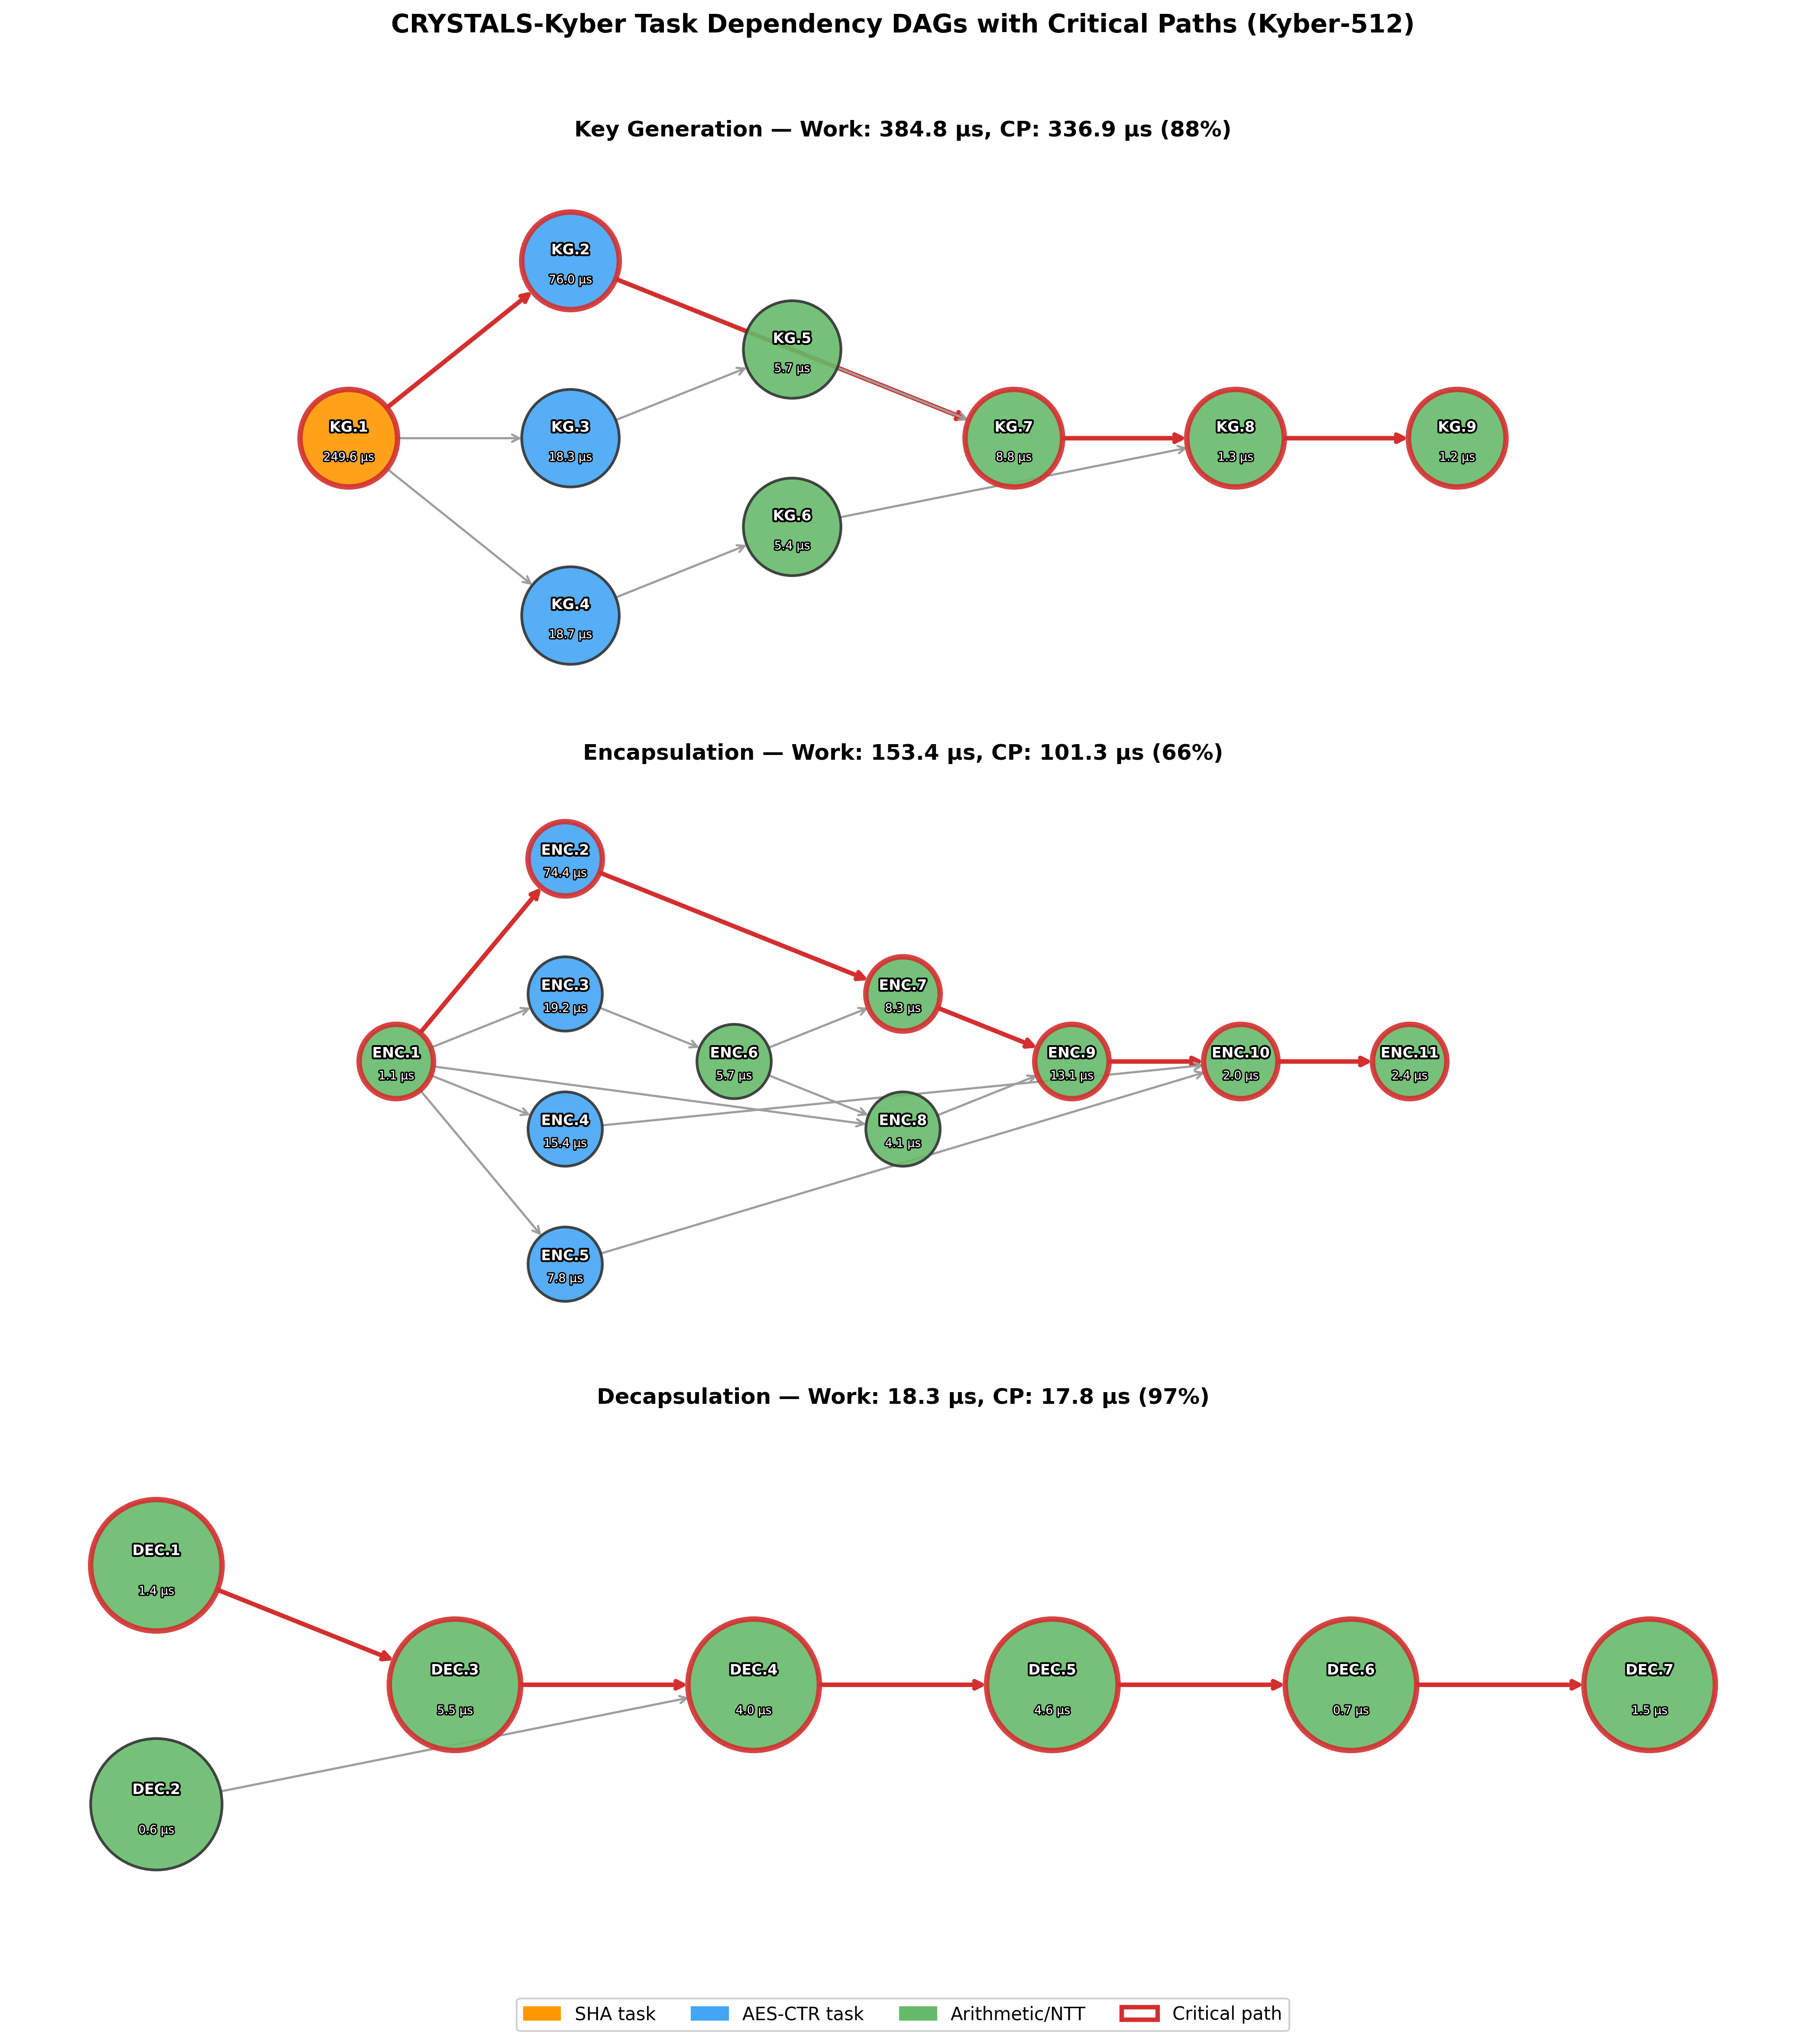
\includegraphics[width=\textwidth]{../sim/results/dag_combined.png}
\caption{Task dependency DAGs for all three KEM operations (Kyber-512) with critical paths highlighted in red. Node colors indicate task type: orange = SHA, blue = AES-CTR, green = arithmetic/NTT. Node labels show task weight in $\mu$s. The critical path consumes 87.5\% of total work in key generation, 66.0\% in encapsulation, and 96.9\% in decapsulation, illustrating the scheduling saturation property.}
\label{fig:dag_combined}
\end{figure*}

\subsection{Sensitivity Analysis Model}
\label{sec:sensitivity_model}

To predict scheduling behavior under hardware acceleration without requiring on-chip measurements, we define a parameterized weight scaling model. For a task $v$ with PC-measured weight $w_{\mathrm{PC}}(v)$ and task category $\mathrm{type}(v) \in \{\text{SHA}, \text{AES}, \text{other}\}$, the accelerated weight is:
\begin{equation}
    w_s(v) = \frac{w_{\mathrm{PC}}(v)}{\alpha_s(\mathrm{type}(v))}
    \label{eq:sensitivity}
\end{equation}
where $\alpha_s$ is a per-category speedup factor parameterized by scenario~$s$:
\begin{itemize}
\item \textbf{Scenario~A:} $\alpha_A(\cdot) = 1$ (no acceleration; PC baseline).
\item \textbf{Scenario~B:} $\alpha_B(\text{SHA}) = 6.1$, $\alpha_B(\text{AES}) = 9.65$ (ESP32 hardware accelerator speedups reported by~\cite{segatz2022}).
\item \textbf{Scenario~C:} $\alpha_C(\text{SHA}) = 4.0$, $\alpha_C(\text{AES}) = 6.0$ (conservative estimate).
\end{itemize}
In all scenarios, $\alpha_s(\text{other}) = 1$ for non-SHA/AES tasks (NTT, polynomial arithmetic, serialization). The scheduling gap metric is defined as:
\begin{equation}
    \mathrm{Gap}(\%) = \frac{M_{\mathrm{Segatz}} - M_{\mathrm{HLFET}}}{M_{\mathrm{HLFET}}} \times 100
    \label{eq:gap}
\end{equation}
where $M_{\mathrm{Segatz}}$ and $M_{\mathrm{HLFET}}$ are the makespans of the Segatz and HLFET schedules, respectively.

\subsection{FIPS 203 Audit Methodology}

The FIPS~203 compliance audit was conducted by systematically comparing each function in the implementation source code against the corresponding algorithm in the FIPS~203 standard document~\cite{fips203}. The audit covered parameter definitions, IND-CPA functions, KEM functions, symmetric primitive bindings, the NTT implementation, and verification utilities. Each deviation was classified by severity (Critical, Moderate, Minor, or Informational) and mapped to a specific FIPS~203 algorithm and step number. Partial fixes addressing the critical and moderate algorithmic gaps were implemented in a separate \texttt{components\_fips203/} directory, preserving the original code for comparison. A Known Answer Test (KAT) suite was developed to validate both versions and confirm divergence.


% ====================================================================
%  5. RESULTS
% ====================================================================
\section{Results}

\subsection{Task Profiling Results}

Table~\ref{tab:profiling} presents the measured average execution times for all 27 sub-tasks of Kyber-512 on the PC simulation platform, averaged over 1000 iterations per task.

\begin{table*}[!t]
\renewcommand{\arraystretch}{1.15}
\caption{Task Execution Times for Kyber-512 (PC Simulation Platform, 1000 Iterations)}
\label{tab:profiling}
\centering
\begin{tabular}{l l r r r r}
\toprule
\textbf{Task} & \textbf{Operation} & \textbf{Avg ($\mu$s)} & \textbf{Min ($\mu$s)} & \textbf{Max ($\mu$s)} & \textbf{\% of Op.} \\
\midrule
KG.1 Seed expansion (SHA-512) & KeyGen & 249.58 & 146.20 & 12087.70 & 64.9 \\
KG.2 Generate matrix $A$ (AES-CTR) & KeyGen & 76.03 & 52.20 & 483.90 & 19.8 \\
KG.3 Noise sampling $\mathbf{s}$ (AES-CTR) & KeyGen & 18.30 & 12.90 & 78.90 & 4.8 \\
KG.4 Noise sampling $\mathbf{e}$ (AES-CTR) & KeyGen & 18.66 & 12.80 & 418.20 & 4.8 \\
KG.5 NTT($\mathbf{s}$) & KeyGen & 5.66 & 3.90 & 79.20 & 1.5 \\
KG.6 NTT($\mathbf{e}$) & KeyGen & 5.36 & 3.70 & 170.00 & 1.4 \\
KG.7 Matrix-vector multiply $A \cdot \hat{s}$ & KeyGen & 8.76 & 6.30 & 49.70 & 2.3 \\
KG.8 Add and reduce & KeyGen & 1.27 & 0.90 & 19.10 & 0.3 \\
KG.9 Pack keys & KeyGen & 1.22 & 0.80 & 21.70 & 0.3 \\
\midrule
ENC.1 Unpack $pk$ & Encaps & 1.06 & 0.70 & 11.40 & 0.7 \\
ENC.2 Generate matrix $A^T$ (AES-CTR) & Encaps & 74.38 & 50.20 & 527.30 & 48.5 \\
ENC.3 Noise sampling $\mathbf{r}$ (AES-CTR) & Encaps & 19.21 & 12.90 & 281.80 & 12.5 \\
ENC.4 Noise sampling $\mathbf{e}_1$ (AES-CTR) & Encaps & 15.37 & 10.40 & 216.60 & 10.0 \\
ENC.5 Noise sampling $\mathbf{e}_2$ (AES-CTR) & Encaps & 7.80 & 5.20 & 165.50 & 5.1 \\
ENC.6 NTT($\mathbf{r}$) & Encaps & 5.65 & 3.90 & 42.20 & 3.7 \\
ENC.7 Matrix-vector multiply $A^T \cdot \hat{r}$ & Encaps & 8.32 & 5.70 & 300.00 & 5.4 \\
ENC.8 Inner product $\hat{t}^T \cdot \hat{r}$ & Encaps & 4.11 & 2.80 & 91.10 & 2.7 \\
ENC.9 Inverse NTT & Encaps & 13.14 & 9.30 & 144.70 & 8.6 \\
ENC.10 Add errors & Encaps & 2.02 & 1.40 & 22.30 & 1.3 \\
ENC.11 Compress and pack & Encaps & 2.38 & 1.60 & 65.50 & 1.6 \\
\midrule
DEC.1 Decompress ciphertext & Decaps & 1.37 & 0.90 & 16.40 & 7.5 \\
DEC.2 Unpack $sk$ & Decaps & 0.56 & 0.30 & 11.70 & 3.1 \\
DEC.3 NTT($\mathbf{u}$) & Decaps & 5.49 & 3.80 & 96.20 & 30.0 \\
DEC.4 Inner product $\hat{s}^T \cdot \hat{u}$ & Decaps & 4.04 & 2.80 & 69.50 & 22.0 \\
DEC.5 Inverse NTT & Decaps & 4.64 & 3.10 & 97.00 & 25.3 \\
DEC.6 Subtract and reduce & Decaps & 0.74 & 0.40 & 30.80 & 4.0 \\
DEC.7 Decode message & Decaps & 1.47 & 0.50 & 695.20 & 8.0 \\
\bottomrule
\end{tabular}
\end{table*}

The profiling reveals extreme weight imbalance across sub-tasks. In key generation, the seed expansion task KG.1 accounts for 249.58~$\mu$s out of a total work of 384.83~$\mu$s (64.9\%), and the matrix generation task KG.2 contributes a further 76.03~$\mu$s (19.8\%). Together, these two SHA/AES tasks account for 84.6\% of key generation time. In encapsulation, the matrix generation task ENC.2 dominates at 74.38~$\mu$s out of 153.43~$\mu$s (48.5\%), with noise sampling tasks ENC.3--ENC.5 collectively contributing 42.38~$\mu$s (27.6\%). Decapsulation exhibits the least weight imbalance with a total work of only 18.32~$\mu$s and contains no SHA or AES operations at the sub-task level, making it insensitive to hardware acceleration.

\subsection{Critical Path Analysis}

The critical path---the longest weighted path through the task dependency DAG---determines the theoretical minimum makespan regardless of the number of available processors. Table~\ref{tab:critical_path} summarizes the analysis for each KEM operation.

\begin{table}[!t]
\renewcommand{\arraystretch}{1.15}
\caption{Critical Path Analysis for Kyber-512}
\label{tab:critical_path}
\centering
\begin{tabular}{l r r r r}
\toprule
\textbf{Operation} & \textbf{Work ($\mu$s)} & \textbf{CP ($\mu$s)} & \textbf{CP/Work} & \textbf{Max $S_p$} \\
\midrule
KeyGen & 384.83 & 336.86 & 87.5\% & 1.14$\times$ \\
Encaps & 153.43 & 101.29 & 66.0\% & 1.51$\times$ \\
Decaps &  18.32 &  17.75 & 96.9\% & 1.03$\times$ \\
\bottomrule
\end{tabular}
\end{table}

The critical path for key generation follows KG.1 $\rightarrow$ KG.2 $\rightarrow$ KG.7 $\rightarrow$ KG.8 $\rightarrow$ KG.9, totaling 336.86~$\mu$s. This path consumes 87.5\% of the total work, leaving only 12.5\% of computation available for parallel execution on a second core. The theoretical maximum speedup is bounded at $384.83 / 336.86 = 1.14\times$.

The critical path for encapsulation follows ENC.1 $\rightarrow$ ENC.2 $\rightarrow$ ENC.7 $\rightarrow$ ENC.9 $\rightarrow$ ENC.10 $\rightarrow$ ENC.11, totaling 101.29~$\mu$s. With a CP/Work ratio of 66.0\%, encapsulation offers the most parallelism, with a theoretical maximum speedup of $1.51\times$.

Decapsulation has the least parallelism, with the critical path consuming 96.9\% of total work. The only task that can execute in parallel is DEC.2 (unpack~$sk$, 0.56~$\mu$s).

These results reveal a structural property of Kyber's task graphs: when the CP/Work ratio exceeds approximately 85\%, the scheduling problem becomes degenerate---any valid assignment that places the critical path tasks on a single core achieves the lower bound. We term this condition \emph{scheduling saturation}. Key generation (87.5\%) and decapsulation (96.9\%) are saturated; encapsulation (66.0\%) is the only operation where scheduling decisions are non-trivial.

\subsection{Scheduling Comparison}

Table~\ref{tab:scheduling} presents the central scheduling comparison under three timing scenarios.

\begin{table*}[!t]
\renewcommand{\arraystretch}{1.15}
\caption{Scheduling Comparison: Segatz vs. HLFET Optimal Across Three Acceleration Scenarios (Kyber-512)}
\label{tab:scheduling}
\centering
\begin{tabular}{l l r r r r}
\toprule
\textbf{Scenario} & \textbf{Operation} & \textbf{Segatz ($\mu$s)} & \textbf{HLFET ($\mu$s)} & \textbf{Gap (\%)} & \textbf{Speedup} \\
\midrule
\multirow{3}{*}{A: PC baseline} & KeyGen & 336.86 & 336.86 & 0.0 & 1.14$\times$ \\
 & Encaps & 101.29 & 101.29 & 0.0 & 1.51$\times$ \\
 & Decaps &  17.75 &  17.75 & 0.0 & 1.03$\times$ \\
\midrule
\multirow{3}{*}{B: HW accel (SHA/$6.1\times$, AES/$9.65\times$)} & KeyGen &  61.66 &  60.05 & 2.7 & 1.25$\times$ \\
 & Encaps &  36.96 &  34.62 & 6.7 & 1.41$\times$ \\
 & Decaps &  17.75 &  17.75 & 0.0 & 1.03$\times$ \\
\midrule
\multirow{3}{*}{C: Conservative (SHA/$4\times$, AES/$6\times$)} & KeyGen &  86.32 &  86.32 & 0.0 & 1.20$\times$ \\
 & Encaps &  39.63 &  39.31 & 0.8 & 1.43$\times$ \\
 & Decaps &  17.75 &  17.75 & 0.0 & 1.03$\times$ \\
\bottomrule
\end{tabular}
\end{table*}

Under Scenario~A, the Segatz schedule achieves optimal makespan for all three operations with a 0.0\% gap. This formally establishes that the Segatz schedule is optimal under software-only timing---not coincidentally, but as a consequence of the scheduling saturation property identified above. Any schedule satisfying the constraint of placing critical-path tasks on one core achieves the lower bound. The 0.0\% gap is a structural property of the task graph, not a property of the Segatz schedule in particular.

\subsection{Sensitivity Analysis}
\label{sec:sensitivity}

The sensitivity analysis reveals the boundary conditions under which structural optimality breaks down. Scenario~B applies the hardware accelerator speedup factors reported by Segatz and Al~Hafiz~\cite{segatz2022}: $6.1\times$ for SHA and $9.65\times$ for AES-CTR. Under these accelerated weights, the Segatz schedule's gap opens to 2.7\% for key generation (61.66~$\mu$s vs.\ optimal 60.05~$\mu$s) and 6.7\% for encapsulation (36.96~$\mu$s vs.\ optimal 34.62~$\mu$s).

The mechanism is clear: hardware acceleration disproportionately shrinks the dominant SHA and AES tasks that formerly constituted the bulk of the critical path, making the remaining arithmetic tasks (NTT, matrix multiplication) relatively more significant. With more balanced task weights, the scheduling assignment matters, and the Segatz assignment is no longer optimal.

Under Scenario~C (conservative acceleration: $4\times$ SHA, $6\times$ AES), the encapsulation gap is 0.8\%, and key generation remains optimal. This confirms that the scheduling gap is a continuous function of the acceleration ratio: it emerges when acceleration is strong enough to rebalance task weights beyond the saturation threshold.

Decapsulation remains optimally scheduled across all scenarios because it contains no SHA or AES tasks and is unaffected by hardware acceleration.

Fig.~\ref{fig:sensitivity} visualizes the scheduling gap across all three scenarios, demonstrating the monotonic relationship between acceleration strength and scheduling suboptimality.

\begin{figure}[!t]
\centering
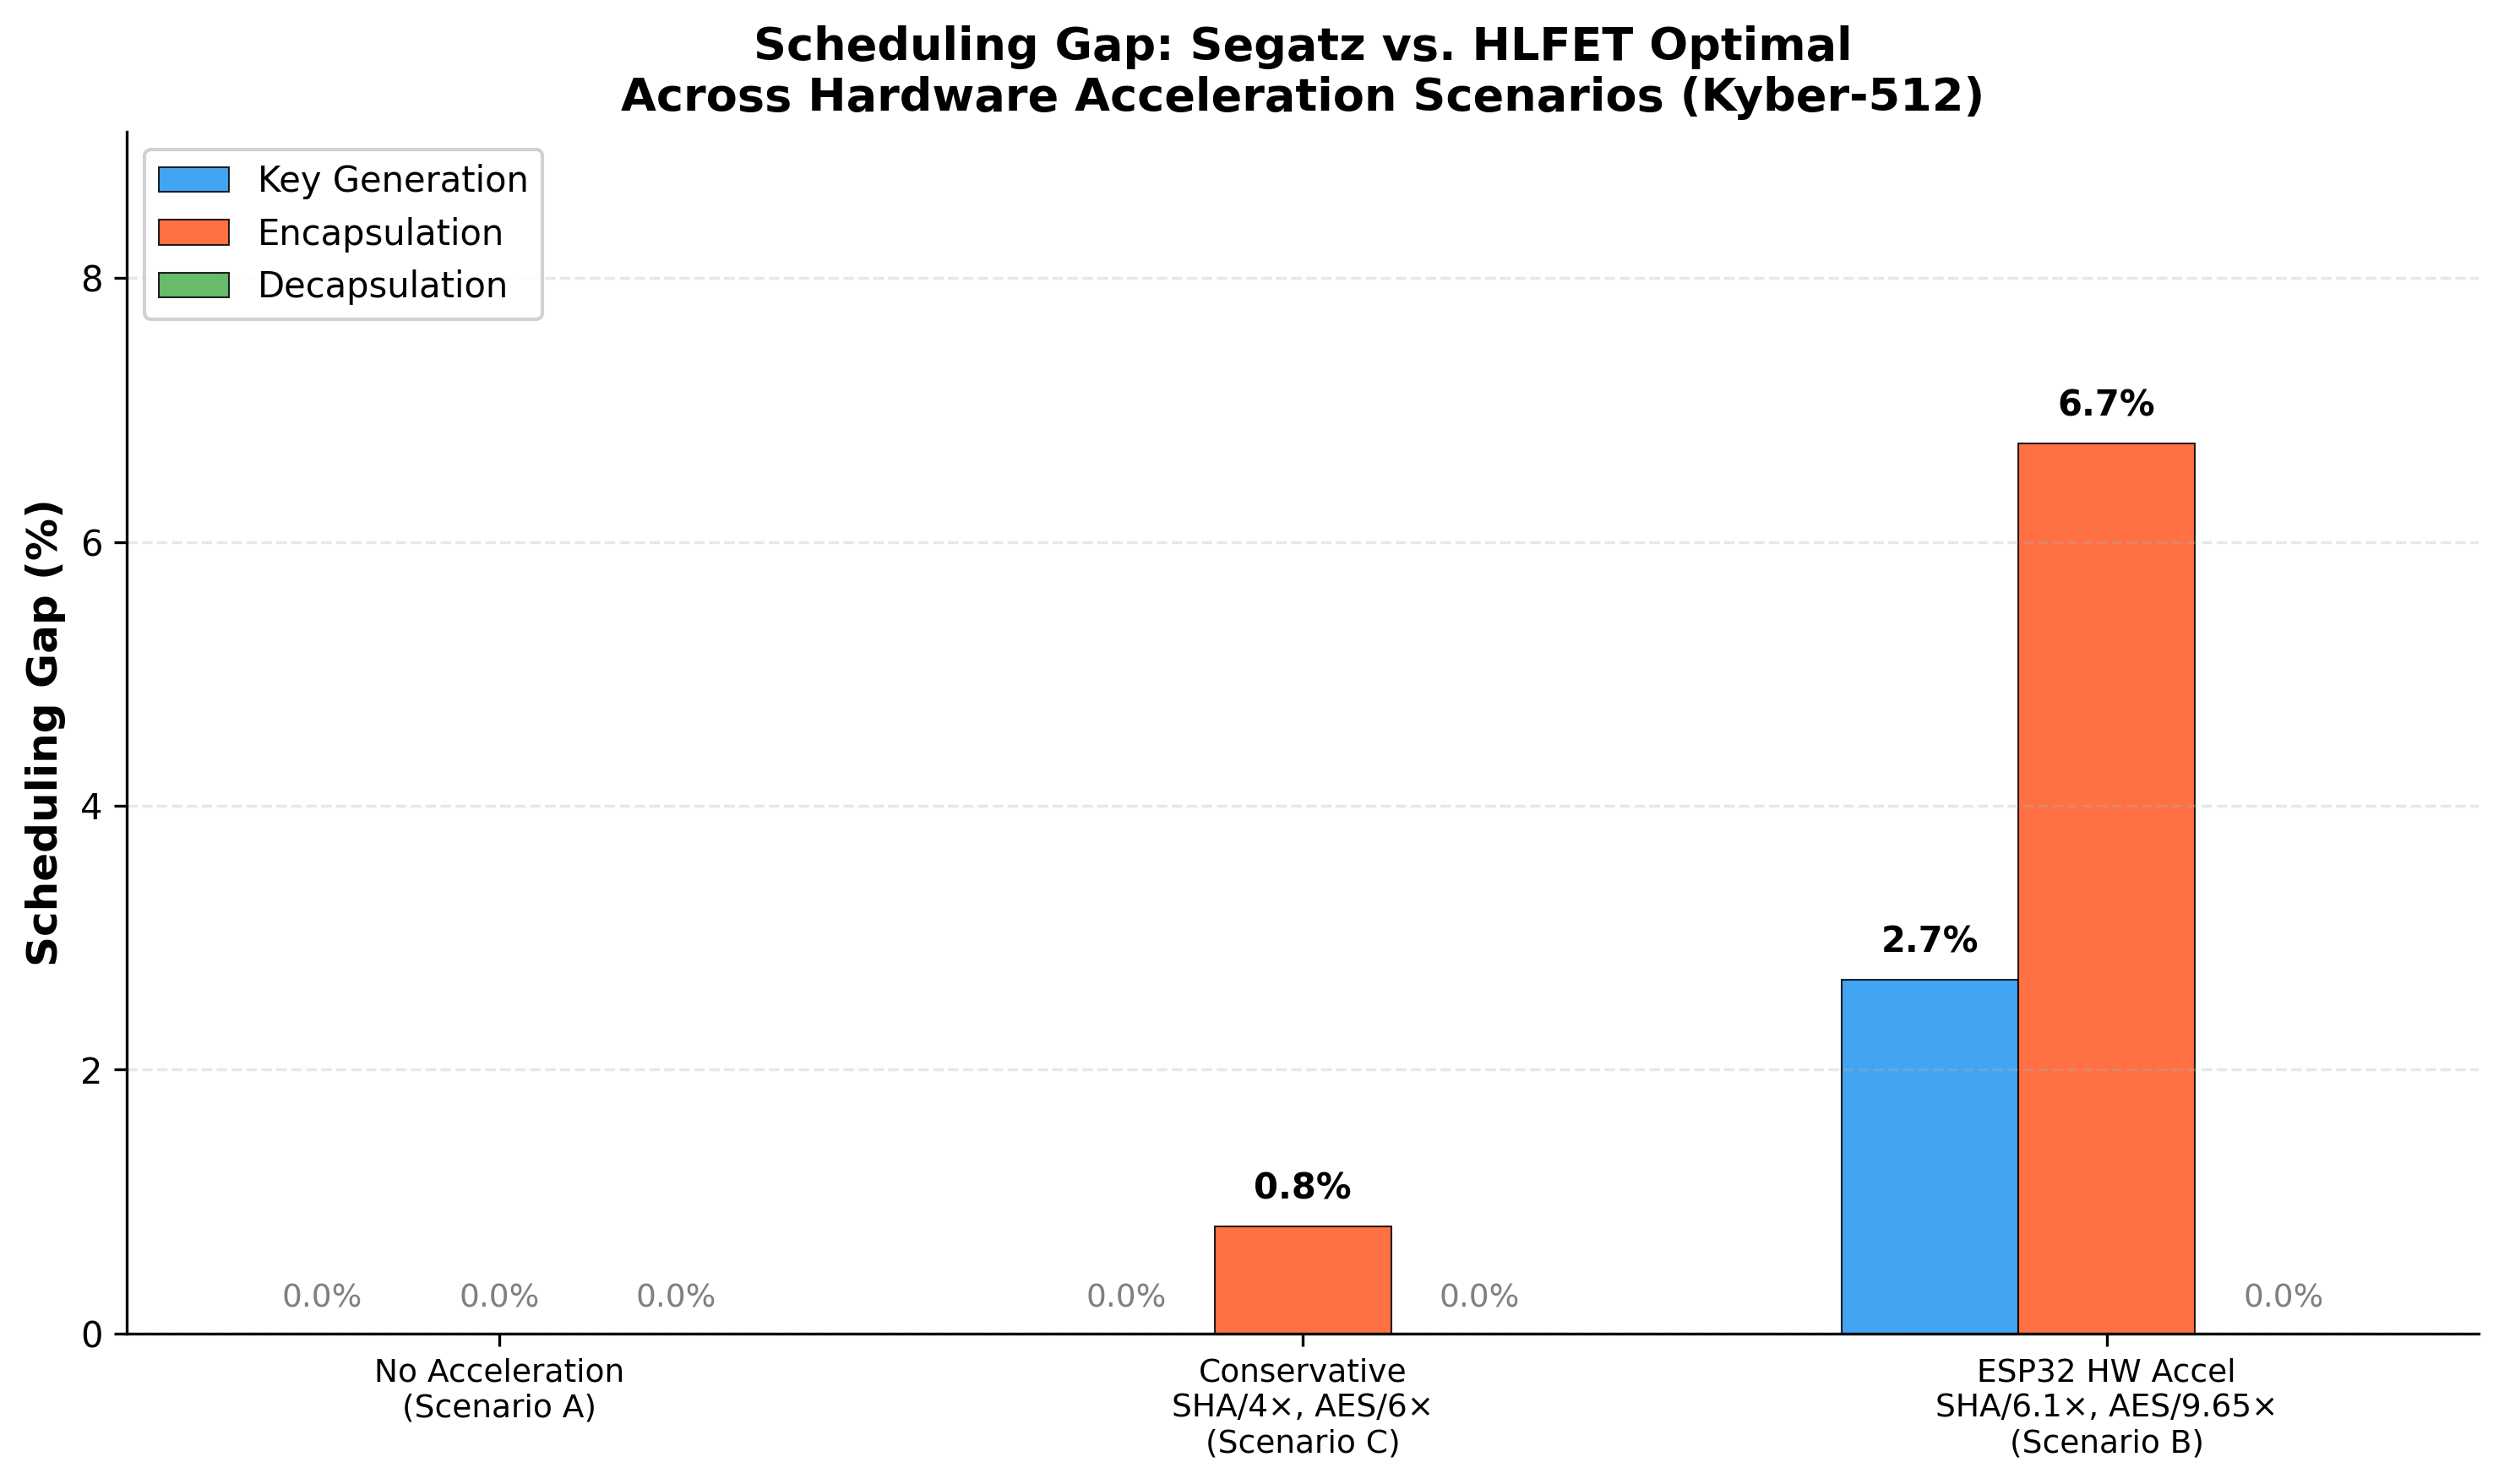
\includegraphics[width=\columnwidth]{../sim/results/sensitivity_plot.png}
\caption{Scheduling gap between Segatz and HLFET-optimal schedules across three hardware acceleration scenarios for Kyber-512. The gap increases monotonically with acceleration strength, reaching 6.7\% for encapsulation under ESP32 hardware acceleration.}
\label{fig:sensitivity}
\end{figure}

\subsection{Schedule Visualization}

Fig.~\ref{fig:gantt_baseline} presents Gantt chart comparisons of the Segatz and HLFET schedules under Scenario~A (baseline timing). The charts confirm the 0.0\% gap: both schedules produce identical makespans for all three operations. The visual dominance of KG.1 (seed expansion) in key generation illustrates why this operation is scheduling-saturated.

\begin{figure*}[!t]
\centering
\includegraphics[width=\textwidth]{../sim/results/optimal_schedule.png}
\caption{Gantt chart comparison: Segatz schedule (left) vs.\ HLFET-optimal schedule (right) for all three KEM operations (Scenario~A: software-only timing, no hardware acceleration). Both schedules achieve identical makespans, confirming the 0.0\% gap.}
\label{fig:gantt_baseline}
\end{figure*}

Fig.~\ref{fig:gantt_scenariob} shows the same comparison under Scenario~B (hardware acceleration). The encapsulation panel clearly shows the 6.7\% gap: the HLFET schedule more efficiently interleaves noise sampling and NTT tasks with the matrix multiplication steps, completing in 34.6~$\mu$s versus the Segatz schedule's 37.0~$\mu$s.

\begin{figure*}[!t]
\centering
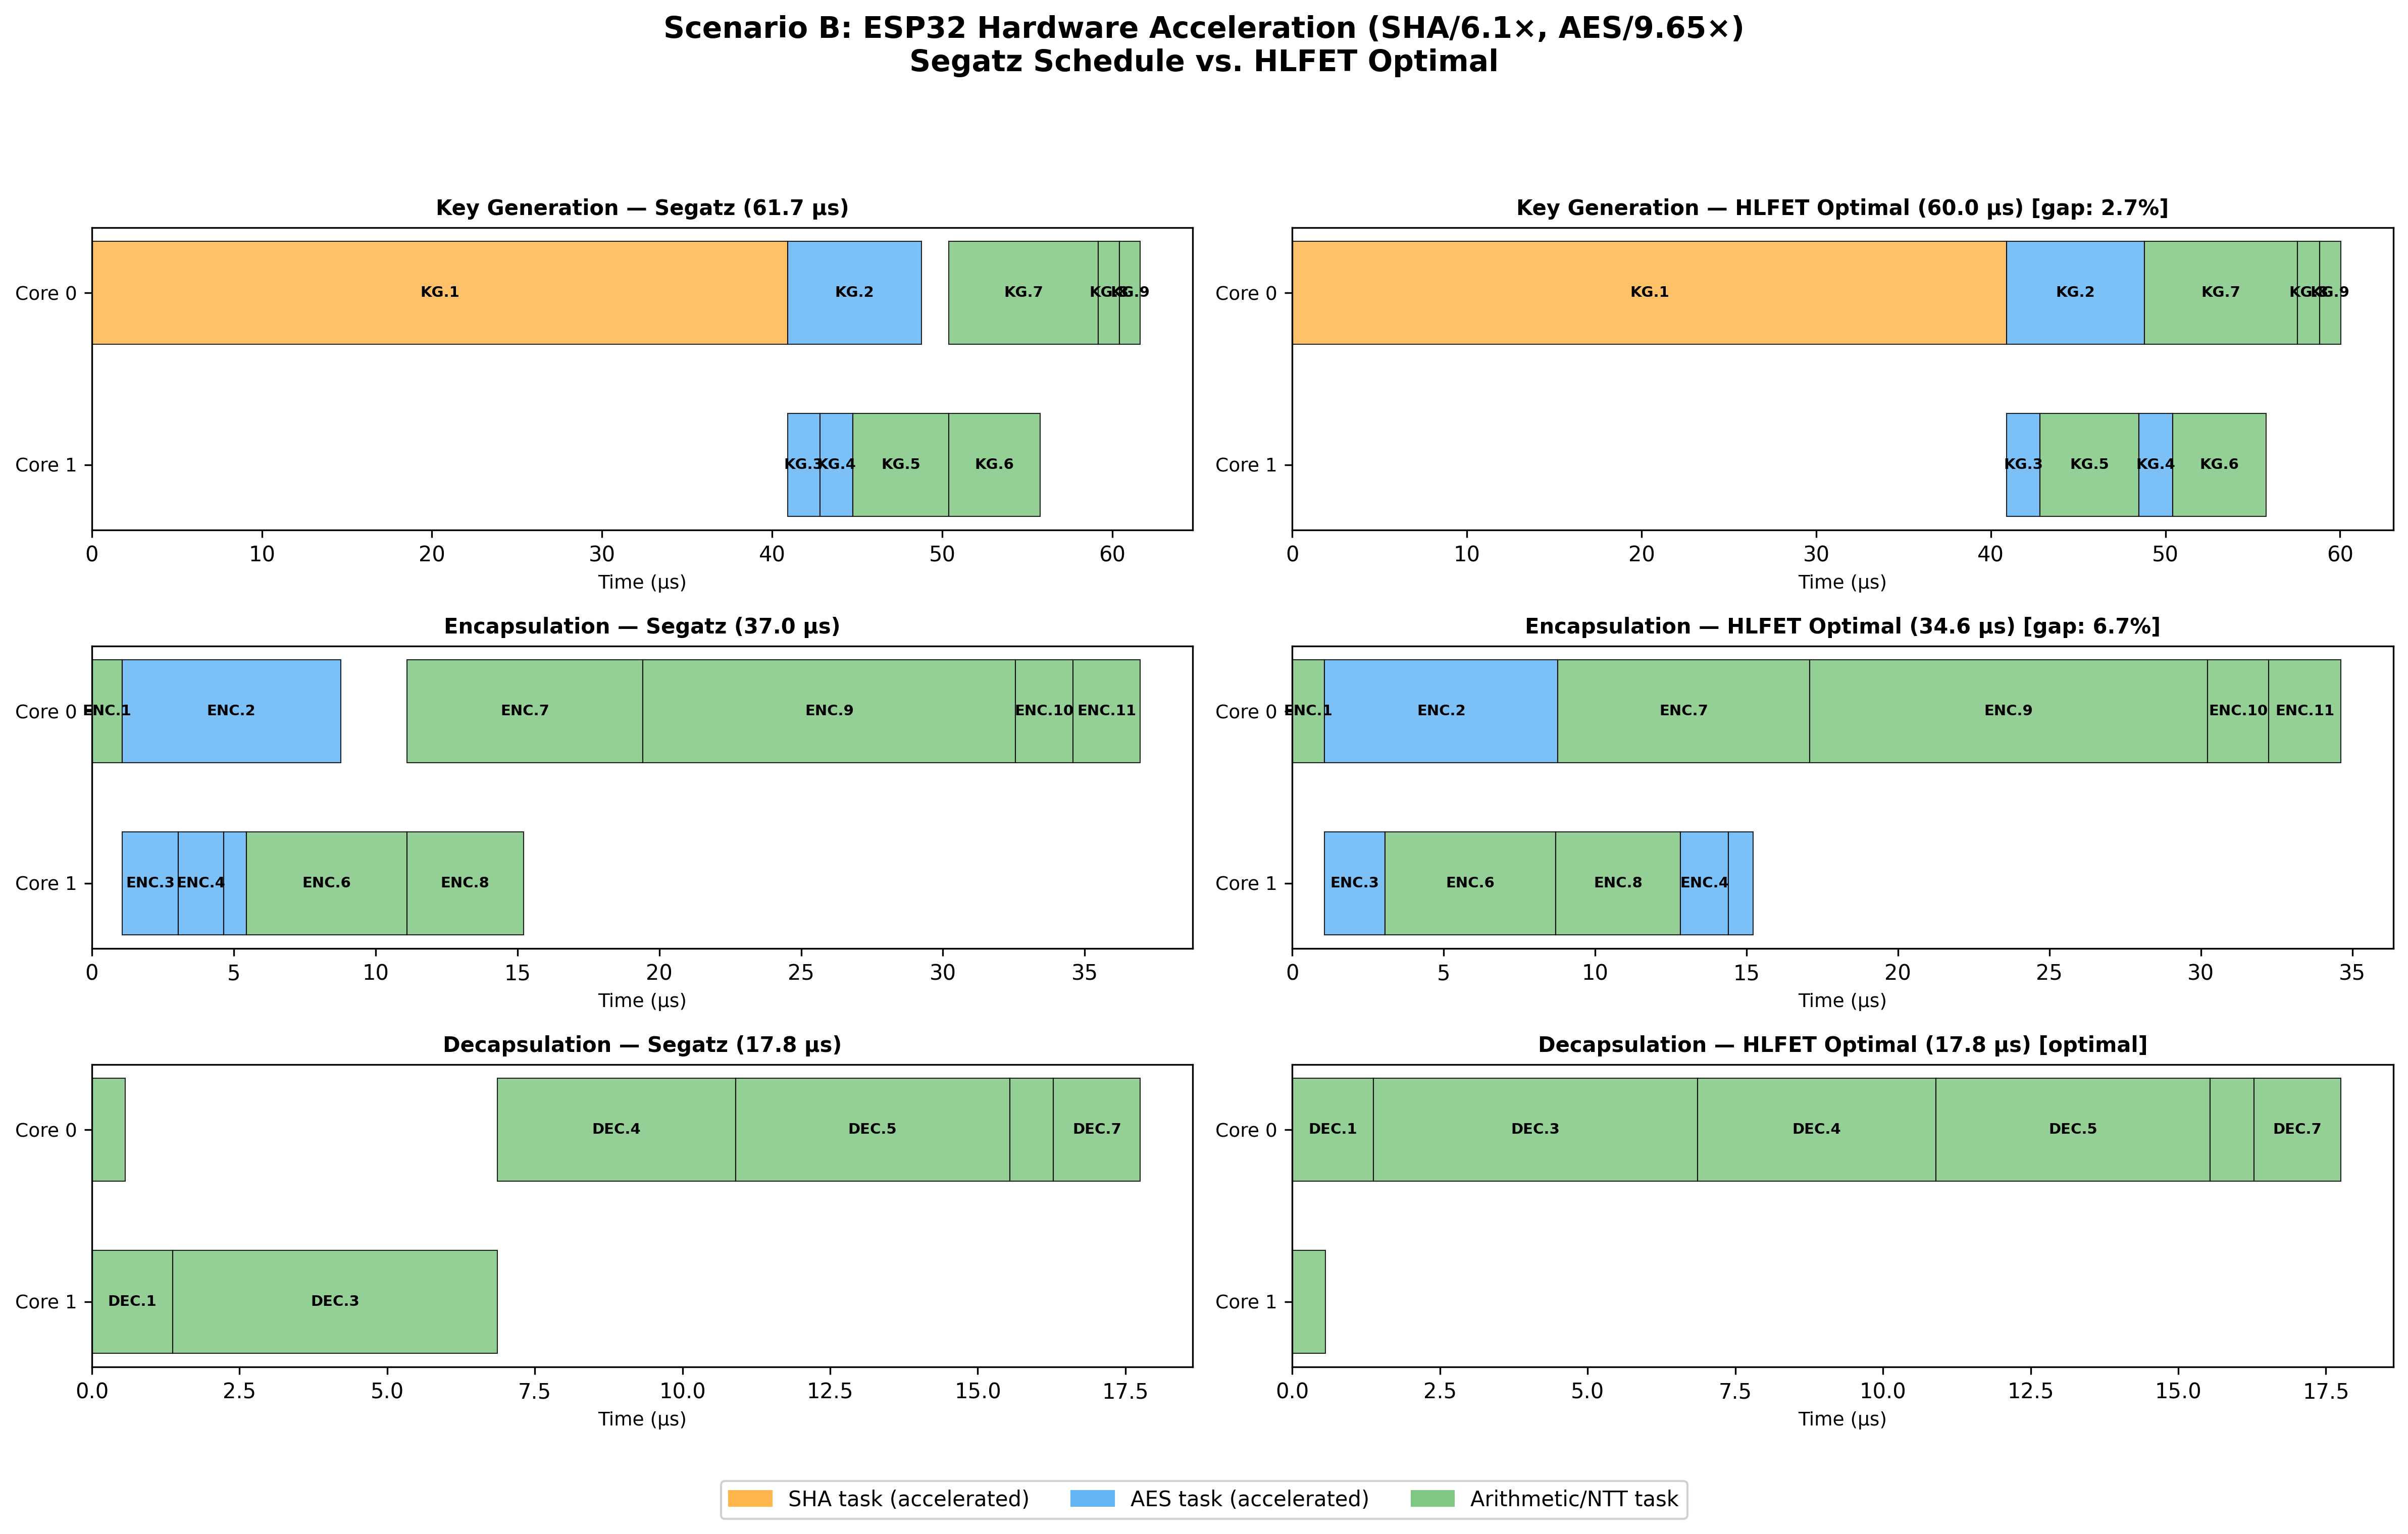
\includegraphics[width=\textwidth]{../sim/results/scenario_b_gantt.png}
\caption{Gantt chart comparison under Scenario~B (ESP32 HW acceleration: SHA/$6.1\times$, AES/$9.65\times$). Task colors indicate type: orange = SHA (accelerated), blue = AES (accelerated), green = arithmetic/NTT. The encapsulation panel shows the 6.7\% gap arising from suboptimal task placement in the Segatz schedule.}
\label{fig:gantt_scenariob}
\end{figure*}



\subsection{FIPS 203 Gap Analysis}

The compliance audit identified nine gaps between the implementation and FIPS~203, summarized in Table~\ref{tab:fips_gaps}.

\begin{table*}[!t]
\renewcommand{\arraystretch}{1.15}
\caption{FIPS 203 Compliance Gaps: Implementation vs.\ Finalized ML-KEM Standard}
\label{tab:fips_gaps}
\centering
\begin{tabular}{c l l l}
\toprule
\textbf{ID} & \textbf{Description} & \textbf{Severity} & \textbf{FIPS 203 Reference} \\
\midrule
GAP-1 & Missing $G(d \| k)$ domain separation in K-PKE.KeyGen & Critical & Algorithm 13, Step 1 \\
GAP-2 & Extra $m \leftarrow H(m)$ pre-hash in ML-KEM.Encaps & Critical & Algorithm 17, Step 1 \\
GAP-3 & $\mathrm{KDF}(K' \| H(c))$ instead of direct $K$; missing $J(z \| c)$ & Critical & Algorithms 17--18 \\
GAP-4 & No modulus check on encapsulation key & Moderate & \S7.1, Algorithm 20 \\
GAP-5 & No input length/type validation & Moderate & \S7.1--7.2 \\
GAP-6 & 90s symmetric primitives not standardized & Moderate & \S4.1 \\
GAP-7 & Seed $d$ generated internally, not as parameter & Minor & Algorithms 13, 16 \\
GAP-8 & Uses ``Kyber'' naming instead of ``ML-KEM'' & Minor & Throughout \\
GAP-9 & Secret key layout $dk = dk_{\text{pke}} \| ek \| H(ek) \| z$ & Info.\ & Algorithm 16 (compliant) \\
\bottomrule
\end{tabular}
\end{table*}

The three critical gaps all affect shared secret computation. GAP-1 omits the domain separation byte in key generation, meaning identical seeds produce identical keys across security levels. GAP-2 retains the pre-hash $m \leftarrow H(m)$ that FIPS~203 removed, causing shared secret divergence from conforming implementations. GAP-3 is the most structurally significant: the implementation derives the shared secret through $\mathrm{KDF}(K' \| H(c))$ instead of using $K$ directly, and uses a different implicit rejection construction.

\subsection{Divergence Validation}

The partial fixes in \texttt{components\_fips203/} address GAPs~1--4 at the algorithmic level while retaining the 90s symmetric primitives. Table~\ref{tab:divergence} summarizes the divergence testing results.

\begin{table}[!t]
\renewcommand{\arraystretch}{1.15}
\caption{KAT Divergence Testing Results}
\label{tab:divergence}
\centering
\begin{tabular}{l c c c}
\toprule
\textbf{Test} & \textbf{$k=2$} & \textbf{$k=3$} & \textbf{$k=4$} \\
\midrule
Public key divergence & 20/20 & 20/20 & 20/20 \\
Shared secret divergence & 20/20 & 20/20 & 20/20 \\
Original round-trip & Pass & Pass & Pass \\
Corrected round-trip & Pass & Pass & Pass \\
\bottomrule
\end{tabular}
\end{table}

The divergence test confirms that the original and FIPS~203-corrected versions produce different public keys in 20/20 trials and different shared secrets in 20/20 trials across all three parameter sets. Both versions independently pass round-trip consistency (encapsulation followed by decapsulation yields the same shared secret).


% ====================================================================
%  6. DISCUSSION
% ====================================================================
\section{Discussion}

\subsection{Scheduling Saturation as a Structural Finding}

The scheduling analysis reveals that the bottleneck in dual-core Kyber is structural, not scheduling-related. Under software-only timing, the critical path through seed expansion and matrix generation is so dominant that it leaves insufficient parallel work to benefit from scheduling optimization. The Segatz schedule is optimal not because of careful scheduling decisions but because the scheduling saturation condition makes virtually any valid schedule optimal.

This finding connects directly to an observation by Segatz and Al~Hafiz~\cite{segatz2022}, who identified matrix $A$ generation as a candidate for future optimization due to its outsized contribution to latency. Our formal analysis provides the theoretical framework to explain \emph{why} this task dominates scheduling behavior: when a single task exceeds approximately 50\% of total work and lies on the critical path, the CP/Work ratio approaches unity and scheduling saturation occurs.

\subsection{The Sensitivity Model as an Analytical Contribution}

The sensitivity analysis constitutes an analytical model of hardware acceleration, not an empirical measurement. The model, defined by~(\ref{eq:sensitivity}), scales task weights within each hardware-accelerated category, parameterized by the speedup ratios~$\alpha_s$. This enables systematic analysis of how scheduling optimality degrades as a function of acceleration ratio, identifying the threshold beyond which empirical schedules become suboptimal.

The model makes a falsifiable prediction: the scheduling gap for encapsulation under ESP32 hardware acceleration is approximately 6.7\%, recoverable through adoption of the HLFET-optimal task assignment. This prediction is testable through on-hardware implementation. The 6.7\% gap represents a concrete scheduling improvement opportunity: the HLFET list scheduler finds a task assignment that completes 2.34~$\mu$s earlier than the Segatz assignment by more efficiently interleaving noise sampling and NTT tasks with matrix multiplication steps.

From a practical standpoint, in high-throughput IoT scenarios where a device performs thousands of encapsulations (e.g., a gateway establishing sessions with multiple clients), cumulative savings become meaningful. More broadly, the result demonstrates that scheduling analysis should be revisited whenever the underlying execution weights change---whether due to hardware acceleration, algorithmic optimization, or platform migration.

\subsection{FIPS 203 Compliance Implications}

The FIPS~203 findings have immediate practical implications. Any device running the current implementation cannot establish shared secrets with a server implementing standardized ML-KEM. The three critical gaps cause output divergence at every stage: key generation produces different public keys (GAP-1), encapsulation produces different shared secrets (GAPs~2 and~3), and decapsulation uses a different implicit rejection mechanism (GAP-3).

For IoT devices being deployed today that must interoperate with modern TLS~1.3 stacks incorporating ML-KEM~\cite{buerstinghaus2020}, this incompatibility is a deployment blocker. The gap taxonomy established by this audit---with severity classification and FIPS~203 algorithm-level citations---is a reusable artifact applicable to any implementation derived from the 2022 pq-crystals reference codebase.

\subsection{Combined Implications}

The two analyses jointly indicate that the implementation requires two categories of updates for continued relevance. First, the task-to-core assignment should be revisited with hardware-accurate timing weights, particularly for encapsulation. Second, the KEM-layer algorithms must be updated to match FIPS~203, and the 90s symmetric primitives should be migrated to SHA-3/SHAKE for full compliance. These two updates are largely independent: the scheduling optimization operates at the sub-task level within K-PKE, while the FIPS~203 compliance fixes operate at the KEM wrapper level.


% ====================================================================
%  7. LIMITATIONS
% ====================================================================
\section{Limitations}

Task execution times were measured on a PC platform (Windows, x86-64) rather than on ESP32 hardware. The DAG structure and dependency relationships are platform-independent; only the absolute and relative task weights differ. The sensitivity analysis addresses this by applying parameterized scaling factors derived from reported accelerator speedups, but these are applied uniformly per task category rather than per individual task.

The FIPS~203 algorithmic fixes retain the 90s symmetric primitives (SHA-2, AES-256-CTR) rather than migrating to SHA-3/SHAKE. They demonstrate the correct algorithmic structure without achieving primitive-level compliance.

The KAT test suite validates internal consistency and confirms inter-version divergence but does not validate against NIST's official ML-KEM test vectors, which require the SHA-3/SHAKE primitive layer.

The HLFET-optimal schedule has not been validated on ESP32 hardware. Implementation would require modifying FreeRTOS task creation and synchronization code, rebuilding firmware, and measuring actual execution times.


% ====================================================================
%  8. CONCLUSION
% ====================================================================
\section{Conclusion}

This paper presented two complementary contributions analyzing the dual-core CRYSTALS-Kyber implementation by Segatz and Al~Hafiz on the ESP32 microcontroller. The first contribution established that their empirical dual-core task assignment is formally optimal under software-only timing weights, achieving a 0.0\% gap relative to the HLFET list scheduling bound for all three KEM operations: key generation (336.86~$\mu$s, $1.14\times$ speedup), encapsulation (101.29~$\mu$s, $1.51\times$ speedup), and decapsulation (17.75~$\mu$s, $1.03\times$ speedup). This optimality was attributed to \emph{scheduling saturation}---a structural property of Kyber's task graphs wherein the CP/Work ratio exceeds 85\%, rendering scheduling decisions trivially satisfied.

A parameterized sensitivity analysis incorporating ESP32 hardware accelerator speedup factors ($6.1\times$ for SHA, $9.65\times$ for AES) revealed that this structural optimality breaks down under hardware acceleration, with the scheduling gap reaching 6.7\% for encapsulation (36.96~$\mu$s Segatz vs.\ 34.62~$\mu$s optimal) and 2.7\% for key generation (61.66~$\mu$s vs.\ 60.05~$\mu$s).

The second contribution identified nine compliance gaps between the implementation and the finalized FIPS~203 (ML-KEM) standard, including three critical algorithmic differences that prevent interoperation with any conforming implementation. Partial fixes were validated through divergence testing, confirming 20/20 output divergence across all three parameter sets.

Future work should pursue three directions. First, the HLFET-optimal schedule should be implemented in the ESP32 firmware and validated with hardware timing measurements to confirm the predicted 6.7\% improvement. Second, the symmetric primitive layer should be migrated from the 90s variant to the FIPS~203-mandated primitives (SHA-3, SHAKE) to achieve full standards compliance. Third, the observation that matrix $A$ generation dominates the critical path across all scenarios suggests that algorithmic optimization of this step would yield larger speedup improvements than any scheduling rearrangement.

This work demonstrates that formal scheduling analysis provides insights not available from empirical implementation alone: it identifies the structural conditions under which scheduling optimization is meaningful, predicts the impact of hardware changes before implementation, and provides a reproducible analytical framework applicable to any dual-core embedded cryptographic implementation.


% ====================================================================
%  ACKNOWLEDGMENT
% ====================================================================
\section*{Acknowledgment}

The authors thank Dr.\ Ritam Sharma for supervision and guidance throughout this project, and the Indian Institute of Information Technology Kota for providing the research environment and resources.


% ====================================================================
%  REFERENCES
% ====================================================================
\begin{thebibliography}{32}

\bibitem{segatz2022}
F.~Segatz and M.~I.~A.~Al~Hafiz, ``Efficient implementation of CRYSTALS-KYBER key encapsulation mechanism on ESP32,'' \emph{arXiv preprint arXiv:2503.10207 [cs.CR]}, 2022.

\bibitem{kyber2021}
R.~Avanzi \emph{et~al.}, ``CRYSTALS-KYBER algorithm specifications and supporting documentation (version 3.02),'' NIST Post-Quantum Cryptography Standardization, Round~3 Submission, 2021.

\bibitem{nist2022announce}
National Institute of Standards and Technology, ``NIST announces first four quantum-resistant cryptographic algorithms,'' NIST News, Jul.\ 2022. [Online]. Available: \url{https://www.nist.gov/news-events/news/2022/07/nist-announces-first-four-quantum-resistant-cryptographic-algorithms}

\bibitem{fips203}
National Institute of Standards and Technology, ``FIPS 203: Module-lattice-based key-encapsulation mechanism standard,'' Federal Information Processing Standards Publication 203, Aug.\ 2024. [Online]. Available: \url{https://doi.org/10.6028/NIST.FIPS.203}

\bibitem{pqcrystals}
J.~Bos \emph{et~al.}, ``pq-crystals/kyber: Reference implementation,'' GitHub. [Online]. Available: \url{https://github.com/pq-crystals/kyber}

\bibitem{shor1999}
P.~W.~Shor, ``Polynomial-time algorithms for prime factorization and discrete logarithms on a quantum computer,'' \emph{SIAM Review}, vol.~41, no.~2, pp.~303--332, 1999.

\bibitem{langlois2012}
A.~Langlois and D.~Stehl\'{e}, ``Worst-case to average-case reductions for module lattices,'' \emph{Cryptology ePrint Archive}, Paper 2012/090, 2012.

\bibitem{fujisaki1999}
E.~Fujisaki and T.~Okamoto, ``Secure integration of asymmetric and symmetric encryption schemes,'' in \emph{Advances in Cryptology---CRYPTO '99}, pp.~537--554, Springer, 1999.

\bibitem{shoup2000}
V.~Shoup, ``Using hash functions as a hedge against chosen ciphertext attack,'' in \emph{Advances in Cryptology---EUROCRYPT 2000}, pp.~275--288, Springer, 2000.

\bibitem{keccak2011}
G.~Bertoni, J.~Daemen, M.~Peeters, and G.~Van~Assche, ``The Keccak reference,'' Submission to the NIST SHA-3 Competition, 2011.

\bibitem{esp32trm}
Espressif Systems, ``ESP32 technical reference manual, version 4.7,'' 2022. [Online]. Available: \url{https://www.espressif.com/sites/default/files/documentation/esp32_technical_reference_manual_en.pdf}

\bibitem{espfreertos}
Espressif Systems, ``ESP-IDF FreeRTOS (SMP).'' [Online]. Available: \url{https://docs.espressif.com/projects/esp-idf/en/release-v5.0/esp32s3/api-guides/freertos-smp.html}

\bibitem{mbedtls}
Arm Limited, ``MbedTLS---TLS API references and tutorials,'' Mbed OS 6 Documentation, 2022.

\bibitem{freertos}
FreeRTOS, ``API reference: Semaphores.'' [Online]. Available: \url{https://www.freertos.org/a00113.html}

\bibitem{buerstinghaus2020}
K.~B\"{u}rstinghaus-Steinbach, C.~Krau\ss, R.~Niederhagen, and M.~Schneider, ``Post-quantum TLS on embedded systems: Integrating and evaluating Kyber and SPHINCS+ with Mbed TLS,'' in \emph{Proc.\ 15th ACM Asia Conf.\ Computer and Communications Security (ASIA CCS '20)}, pp.~841--852, ACM, 2020.

\bibitem{wang2020}
B.~Wang, X.~Gu, and Y.~Yang, ``Saber on ESP32,'' in \emph{Applied Cryptography and Network Security (ACNS 2020)}, pp.~421--440, Springer, 2020.

\bibitem{botros2019}
L.~Botros, M.~J.~Kannwischer, and P.~Schwabe, ``Memory-efficient high-speed implementation of Kyber on Cortex-M4,'' in \emph{Progress in Cryptology---AFRICACRYPT 2019}, pp.~209--228, Springer, 2019.

\bibitem{pqm4}
M.~J.~Kannwischer, R.~Petri, J.~Rijneveld, P.~Schwabe, and K.~Stoffelen, ``PQM4: Post-quantum crypto library for the ARM Cortex-M4,'' GitHub. [Online]. Available: \url{https://github.com/mupq/pqm4}

\bibitem{heinz2022}
D.~Heinz \emph{et~al.}, ``First-order masked Kyber on ARM Cortex-M4,'' \emph{Cryptology ePrint Archive}, 2022/058, 2022.

\bibitem{ni2022}
Z.~Ni, A.~Khalid, D.~S.~Kundi, M.~O'Neill, and W.~Liu, ``Efficient pipelining exploration for a high-performance CRYSTALS-Kyber accelerator,'' \emph{Cryptology ePrint Archive}, Paper 2022/1093, 2022.

\bibitem{schoffel2022}
M.~Sch\"{o}ffel, F.~Lauer, C.~C.~Rheinl\"{a}nder, and N.~Wehn, ``Secure IoT in the era of quantum computers---where are the bottlenecks?'' \emph{Sensors}, vol.~22, no.~7, p.~2484, 2022.

\bibitem{buchmann2017}
J.~Buchmann, K.~Lauter, and M.~Mosca, ``Postquantum cryptography---state of the art,'' \emph{IEEE Security \& Privacy}, vol.~15, no.~4, pp.~12--13, 2017.

\bibitem{diffie1976}
W.~Diffie and M.~Hellman, ``New directions in cryptography,'' \emph{IEEE Trans.\ Inform.\ Theory}, vol.~22, no.~6, pp.~644--654, 1976.

\bibitem{nist2022status}
G.~Alagic \emph{et~al.}, ``Status report on the third round of the NIST post-quantum cryptography standardization process,'' NIST Internal Report, 2022.

\bibitem{kwok1999}
Y.-K.~Kwok and I.~Ahmad, ``Static scheduling algorithms for allocating directed task graphs to multiprocessors,'' \emph{ACM Computing Surveys}, vol.~31, no.~4, pp.~406--471, 1999.

\bibitem{coffman1972}
E.~G.~Coffman and R.~L.~Graham, ``Optimal scheduling for two-processor systems,'' \emph{Acta Informatica}, vol.~1, no.~3, pp.~200--213, 1972.

\bibitem{graham1969}
R.~L.~Graham, ``Bounds on multiprocessing timing anomalies,'' \emph{SIAM J.\ Applied Mathematics}, vol.~17, no.~2, pp.~416--429, 1969.

\bibitem{topcuoglu2002}
H.~Topcuoglu, S.~Hariri, and M.~Wu, ``Performance-effective and low-complexity task scheduling for heterogeneous computing,'' \emph{IEEE Trans.\ Parallel \& Distributed Systems}, vol.~13, no.~3, pp.~260--274, 2002.

\bibitem{adam1974}
T.~L.~Adam, K.~M.~Chandy, and J.~R.~Dickson, ``A comparison of list schedules for parallel processing systems,'' \emph{Commun.\ ACM}, vol.~17, no.~12, pp.~685--690, 1974.

\bibitem{segatz2022repo}
F.~Segatz and M.~I.~A.~Al~Hafiz, ``kybesp32: Kyber on ESP32,'' GitHub. [Online]. Available: \url{https://github.com/fsegatz/kybesp32}

\bibitem{maier2017}
A.~Maier, A.~Sharp, and Y.~Vagapov, ``Comparative analysis and practical implementation of the ESP32 microcontroller module for the Internet of Things,'' in \emph{2017 Internet Technologies and Applications (ITA)}, pp.~143--148, IEEE, 2017.

\bibitem{takagi2016}
T.~Takagi, \emph{Post-Quantum Cryptography}, Lecture Notes in Computer Science, vol.~9606, Springer, 2016.

\end{thebibliography}


% ====================================================================
%  BIOGRAPHIES
% ====================================================================
\begin{IEEEbiographynophoto}{Karan Sonawane}
(2023KUCP1153) is a B.Tech student in Computer Science and Engineering at the Indian Institute of Information Technology Kota, Rajasthan, India. His research interests include post-quantum cryptography, embedded systems security, and parallel computing on resource-constrained platforms.
\end{IEEEbiographynophoto}

\begin{IEEEbiographynophoto}{Achyut Gupta}
(2023KUCP1158) is a B.Tech student in Computer Science and Engineering at the Indian Institute of Information Technology Kota, Rajasthan, India. His research interests include cryptographic protocol analysis and IoT security.
\end{IEEEbiographynophoto}

\begin{IEEEbiographynophoto}{Bhavesh}
(2023KUCP1159) is a B.Tech student in Computer Science and Engineering at the Indian Institute of Information Technology Kota, Rajasthan, India. His research interests include formal methods and embedded systems.
\end{IEEEbiographynophoto}

\end{document}
